\chapter{Survey}
\label{chp:amtsurvey} 

To be able to map to what extent people care and are aware of their Facebook settings, regarding privacy, security and interdependent privacy, we designed and distributed a survey. The survey addressed the different settings available on Facebook, and awareness regarding Facebook applications and knowledge about interdependent privacy. For the design of the survey, we utilized SurveyMonkey which provides web-based survey solutions (see section \ref{sec:sm}). We distributed the survey on two platforms, namely Amazon Mechanical Turk (AMT) and Facebook. Amazon Mechanical Turk is a Internet marketplace where human intelligence is utilized to perform various tasks \cite{amazonweb}. For more information about Amazon Mechanical Turk, see section \ref{sec:amt}. To reach out to a even larger audience, we posted the survey-link on our Facebook pages. In this chapter we will describe how we designed the survey, how it is structured and how we distributed our survey. We will examine the results with focus on interdependent privacy. 


\section{Constructing the Survey}
There is not much research on the area of interdependent privacy. To be able to bring forward information and contribute to new research, we created a survey. When making the questions, we wanted to create an image of peoples use of Facebook, how they set their settings and how they know and care about their privacy and to what extent their privacy is dependent on other users. We quickly chose to use AMT as a platform for distributing the survey, because we wanted to create an image of the average Facebook user as well as getting a high diversity among the respondents (different countries, age, education etc.). Previous research shows positive results with the use of AMT \cite{expectations,incentivesAmt}. 

\paragraph{}
We started implementing the survey inside the survey template provided by AMT. After some consideration, we found that AMT did fulfil our requirements for design, so we chose to implement the survey using SurveyMonkey instead. When creating the survey, we thought that it would be better to include some extra questions, than to leave some behind. When the survey first got distributed, we were not longer able to edit the questions. We therefore chose to include questions not only regarding privacy and interdependent privacy, but also other aspects of Facebook usage. For example some questions about security settings, usage, personal experience in regard to photos and comment sharing.

\subsection{Design}
AMT offers a template for creating surveys. This template uses HTML. It is simple, but requires more work from the requester. We found the template to be little user friendly, and it did not give you many design options. Our survey consist of many questions, and some of them had follow-up questions requiring text answers. It was then desirable to have these on two different pages. We did not want the respondents to have their answers affected by the next question. It requires more of the respondent to write a text answer, so to avoid them answering based on the next question we separated the questions onto different pages. For example, we have one question asking whether or not the use of Facebook has lead to any uncomfortable situations. If the user answers "Yes", a follow-up question asking to describe the situation that occurred will appear. If the user answers "No" the follow-up question will be skipped. If the user had seen the follow-up question, he/she may not be bothered to answer yes even though this may have been the truthful answer. We did not find an easy solution to implement this design feature in AMT, so we looked for other options. Even though AMT provides their own "Survey"-template, they also provide a "Survey Link"-template. This means that you can create the survey somewhere else, and just link to it in AMT. We chose the latter, and used SurveyMonkey to create the survey. SurveyMonkey provided us with the tools and features necessary to design our survey as desired. 

\paragraph{Features we used in SurveyMonkey.}
SurveyMonkey offers several features, and has a intuitive user interface. It was easy to implement the questions, and separate them on different pages which was of high value to us. SurveyMonkey offers the ability to customize the appearance (color/theme, layout, etc.) of the survey to a higher extent than AMT. We put in a picture of the university logo, to emphasize the seriousness of the survey, as shown in \fref{fig:frontpage}. SurveyMonkey also offers many different question types (multiple choice, text box, matrix and drop-down menus, etc.), and restrictions on the questions. It was important to have some restrictions especially on the text boxes. Some of the restrictions that we used was to limit the amount of characters in the text boxes, to avoid too long answers. We also made almost all questions mandatory, meaning that the respondents had to answer them before being able to move to the next question. As mentioned we divided the questions onto several different pages. This gives the respondents the impression that the survey is shorter. Each page has a title on top, grouping the different areas the questions consider. A progress bar was added to show in percent how far into the survey the respondent was at any time. This gives a good overview, and the user get a feeling of how much is left. We chose to use these features to avoid overwhelming the respondents with too many questions at a time. 

SurveyMonkey offers a great user interface also when it comes to reviewing the answers. It is possible to see graphs showing the distribution of answers to all of the questions, as well as individual answers. SurveyMonkey also offers a filter and comparing feature, which made the analysis a lot easier, especially when having a large number of respondents. 

\subsection{How the Survey is Structured} 
The first page seen when taking the survey, is a introduction page that shortly explains what the survey is about, and it's purpose. This page emphasizes the seriousness of the survey. When people see that it is a research survey carried out by master students at an university, we believe people will answer in a serious manner. The front page also includes the requirement for taking the survey, and a short explanation on where to find answers requested in some of the questions. This is shown in \fref{fig:frontpage}. As mentioned before, we have divided the questions into different areas, and we will now go through each area and emphasize and elaborate the questions we consider as most relevant and important. 
 
\begin{figure}[h!]
\centering
\fbox{
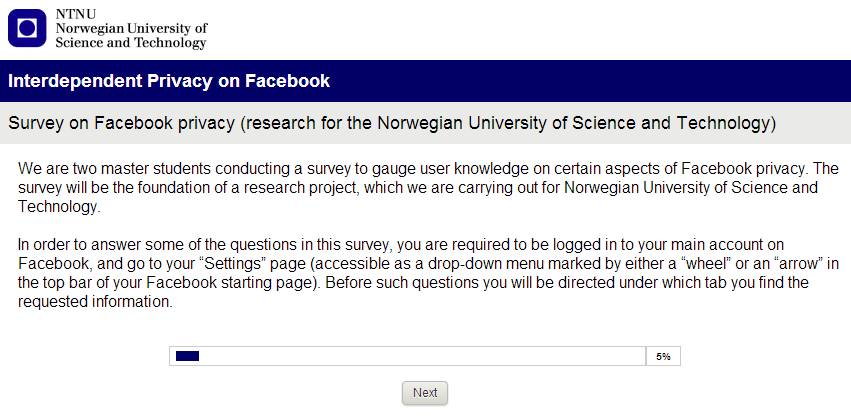
\includegraphics[width=1\textwidth]{firstpagesurvey.png} }
\caption[Front page of the survey]{\textbf{Front page of the survey.} This figure shows the first page of our survey. It gives a short explanation about the purpose of the survey, and what it concerns. It also give some helping guidelines to where to find answers to some of the questions, and the requirement for taking the survey (that you need to be logged in to your main Facebook account).} 
\label{fig:frontpage}
\end{figure}

\subsubsection{Facebook usage}
Following the first page, is one page about Facebook usage. This page includes questions about sign-up year, how often they check their Facebook page and number of friends. 

\subsubsection{Facebook privacy: settings}
This is a part of the survey where the users need to be logged in to their main account on Facebook to check how their privacy settings look. The questions are taken directly from the "Privacy"-settings and "Timeline and tagging"-settings on Facebook. We divided these questions onto 4 different pages. Before we started asking about specific settings, we asked the users how often they have checked their Facebook privacy settings during the last year.  One of the following pages ask for the privacy settings, and another for the timeline and tagging settings. These questions are straightforward for the user, since all they have to do is to render the settings they have set themselves. This will easily show us how many that actually have checked their settings, and to what extent they have made them more, or less, private than default. At the end we asked the users whether or not they consider changing their settings after having reviewed them. This can make for some interesting observations, and can also give an impression of whether or not the users care or are aware of the settings. 

\subsubsection{Facebook privacy: personal experience}

\begin{figure}[h!]
\centering
\fbox{
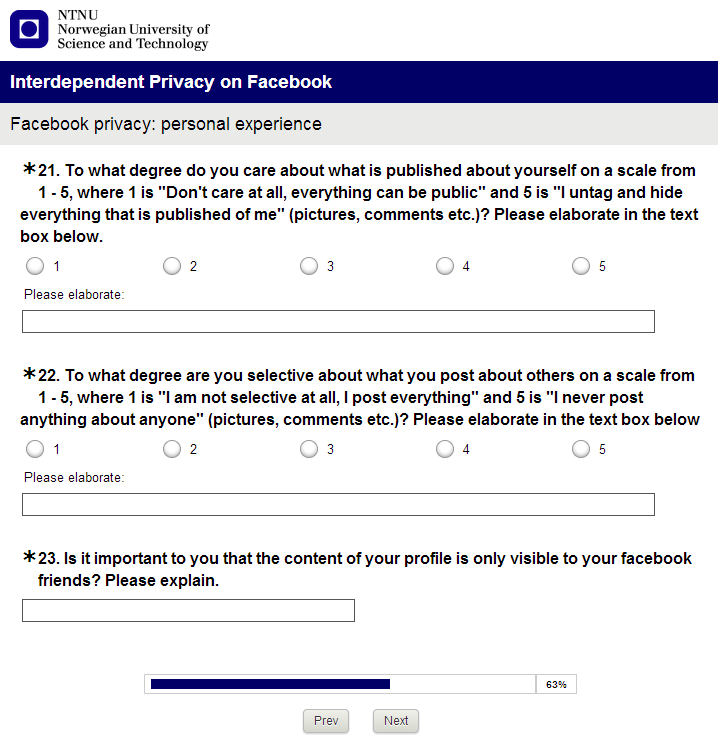
\includegraphics[width=1\textwidth]{page12.png} }
\caption[Question 21 and 22 in the survey]{\textbf{Question 21 and 22 in the survey.} This figure shows question 21 and 22 in the survey. The questions concerns to what degree (on a scale from 1 to 5) the respondents care about what is published about themselves, and what they publish about others. After each of the two questions it is a text box where the respondents can elaborate.} 
\label{fig:page12}
\end{figure}

This group of questions focus on the users personal experience with concern to both privacy and interdependent privacy. We ask whether or not the respondents have experienced that their use of Facebook has affected their professional life or led to any uncomfortable situations. Both of these questions have a follow-up question where the users are asked to describe the situation that occurred. You will only be sent to the page with the follow-up question if you answered yes. If you answered no, the page with the follow-up question will be skipped. 

A big part of Facebook consists of sharing photos and comments with others, we therefore asked the respondents to indicate on a scale from 1 to 5 how much they care about what is published about themselves, and what they publish about others, see \fref{fig:page12}. It was mandatory for the users to give an answer on the scale. We added a text box for the users to elaborate if desired, but this was not mandatory. We received a total of 250 responses on our survey, and 190 of them chose to elaborate. 

\subsubsection{Facebook privacy: apps}
This is the part of the survey that concerns interdependent privacy (see section \ref{sec:intpriv}), and also the most important part of our suvey. As mentioned before this is a relatively unknown term, so we wanted to find out whether or not the respondents knew the meaning of interdependent privacy. Since the app platform on Facebook to a high extent relies on information about a user's friends, it is in this area interdependent privacy becomes more important to address. When you install an app on Facebook, it asks for your basic information, and often more information about you and your friends. For more detailed information about the app-platform, see subsection \ref{subsec:app}. Question 26, 27, 28 and 29 (see \fref{fig:page14} and \fref{fig:page15}) asks about the users awareness regarding what kind of information the apps can retrieve. There exists settings directed towards apps on Facebook (see \fref{fig:apps2013}). In question 30 (\fref{fig:page15}) we ask the user to look at one of the app settings, "Apps others use". In this setting the user decides which information they make available to apps others use, in other words control the categories of information that people can bring with them when they use apps. We want to know if the user are aware of the existence of this setting. We did not ask for more specifics about what information they share, because this is not relevant. What is relevant is whether or not they know it exists, and are aware of what kind of information they share. We finish this part of the survey with the same question we started it with, if they know the meaning of interdependent privacy. We wanted to ask again to see if they got a higher understanding of the term after answering questions about apps, and saw how it is all interconnected. 

\begin{figure}[h!]
\centering
\fbox{
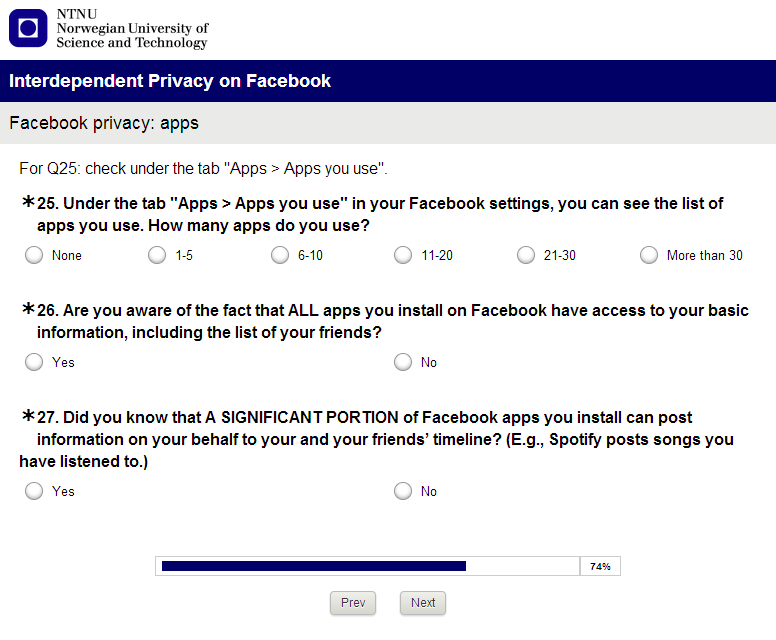
\includegraphics[width=1\textwidth]{page14.png} }
\caption[Question 25, 26 and 27 in the survey]{\textbf{Question 25, 26 and 27 in the survey.} This figure show question 25, 26 and 27 in our survey. Question 25 concern the number of apps the respondents use. Question 26 and 27 concerns the user's awareness connected to apps on Facebook.} 
\label{fig:page14}
\end{figure}

\begin{figure}[h!]
\centering
\fbox{
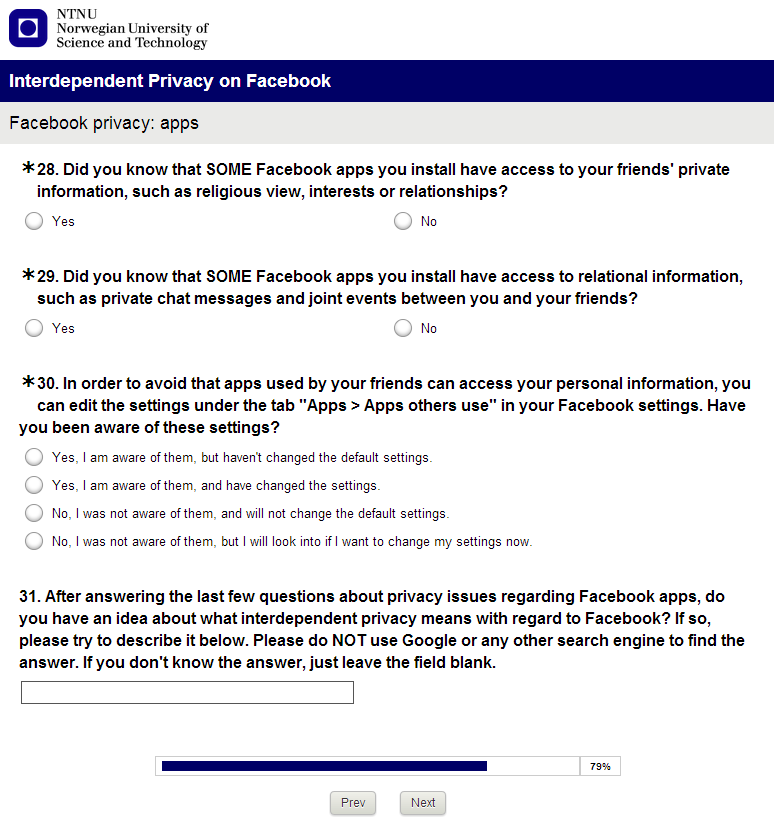
\includegraphics[width=1\textwidth]{page15.png} }
\caption[Question 28, 29, 30 and 31 in the survey]{\textbf{Question 28, 29, 30 and 31 in the survey.} This figure show question 28, 29, 30 and 31 in our survey. Question 28, 29 and 30 concerns the user's awareness connected to apps on Facebook. Question 31 asks the respondents whether or not they know what the term interdependent privacy means after answering questions about apps.} 
\label{fig:page15}
\end{figure}

\subsubsection{Facebook security: settings}
The main focus in this report is on privacy, not security. At the same time, we wanted to ask a few questions regarding Facebook security settings as well. The reason for this is because we wanted to see if there was a connection between strict security settings and strict privacy settings among the respondents of our survey. The questions concerns whether or not the respondents use secure browsing and login notification.

\subsubsection{Demographics}
In the last part of our survey, we have asked for demographic information about the respondents, to get a hunch of what kind of people have taken the survey. We chose to put the demographics part at the end, rather than in the beginning. We assume that a respondents attention span gets lower during the survey, we therefore wanted to put the "easy" questions at the end since they require less focus. These questions consists of: gender, age, country, family situation, highest qualification/degree, employment status and income. Although these questions are easy to answer, they are very important to include. When analysing, they are necessary in order to be able to draw comparisons between for example age and/or gender. An interesting factor is to see where the respondents using AMT come from.  

\subsection{Distributing the Survey}
First we created a requester account on AMT. We did this using an already existing Amazon account. While creating the project (our project contained only one HIT) we filled out the properties shown in \fref{fig:amtedit}. First we had to give a short title and description to describe our HIT to the workers. This is the information that is shown to the workers before they choose to either accept the HIT or skip the HIT. We also had to decide a reward for the workers. We had limited time, and wanted our HIT to be as attractive as possible, and therefore chose to have a higher reward than average. We sat the reward to be \$1.5 per completed assignment. We estimated that it would take approximately 15 minutes to take the survey, this would give a hourly wage of \$6. We were also asked to set a maximum number of assignments per HIT, this means number of unique answers. We sat this number to 250. We felt that 250 responses would give us a very good foundation to base our analysis on. AMT defines a feature that let the requester review the answers, and then choose to either approve or discard them. When discarding an answer, they worker will not get paid. If we did not manually approve the answers, they would automatically be approved after 3 days. We made the HIT available for only 21 days. To get a high quality on the responses, we were advised to use "Master Workers". This is users that have a good reputation from previous work done on AMT. See section \ref{sec:methodology} for more information about "Master Workers". 

\begin{figure}[h!]
\centering
\fbox{
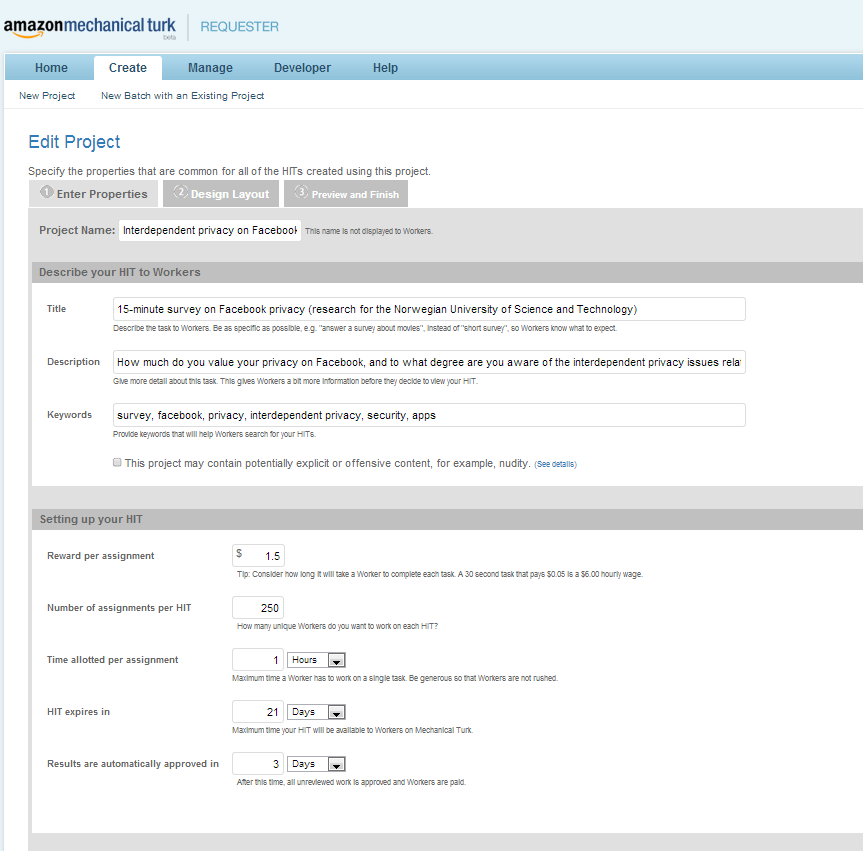
\includegraphics[width=1\textwidth]{amtedit.png} }
\caption[Creating an AMT project]{\textbf{Creating an AMT project.} This figure shows the layout for creating a new project in AMT. Here we stated the title, description, keywords, as well as defining the reward, number of unique workers and expiration date on the HIT.} 
\label{fig:amtedit}
\end{figure}

Next we filled in the "Survey-Link"-template provided by AMT, and the result of this is shown in \fref{fig:amtlayout}. It contains a title and a short description. In the description we linked to the homepage of the Norwegian University of Science and Technology, to emphasize the seriousness of the survey. In addition it contained the link to the survey on SurveyMonkey, as well as a field for the users to enter a survey code. This code was provided to them after they completed the survey. This was an assurance for us, so we only paid the people who actually took the survey. To avoid workers cheating with the code (for example getting the code from a fellow AMT-worker), we changed it several times during it's lifetime. 

\begin{figure}[h!]
\centering
\fbox{
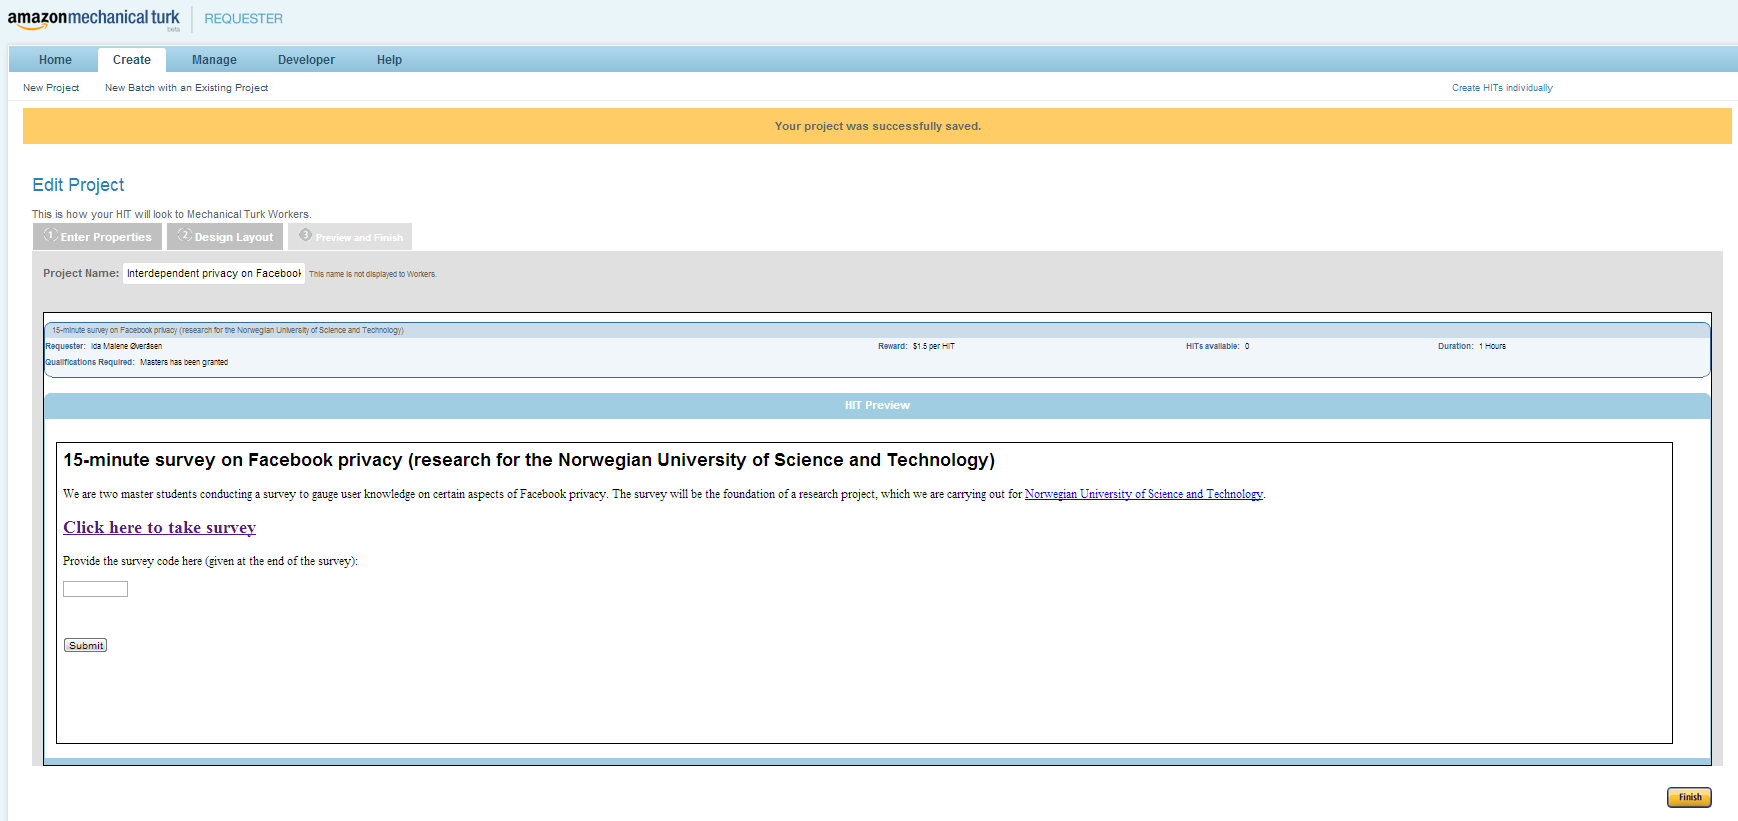
\includegraphics[width=1\textwidth]{amtlayout.png} }
\caption[The design and layout of the survey on AMT]{\textbf{The design and layout of the survey on AMT.} This figure shows the design and layout for the HIT. This is how it looks like for the workers.} 
\label{fig:amtlayout}
\end{figure}

After editing the project as described above, the HIT was ready to be published. The published HIT is shown in \fref{fig:hitout}. After filtering on HITs requiring Master qualification, our HIT is shown at the top. 
Once our HIT was out, all we could do was to monitor it (approve or discard answers), and wait for people to respond. 

\begin{figure}[h!]
\centering
\fbox{
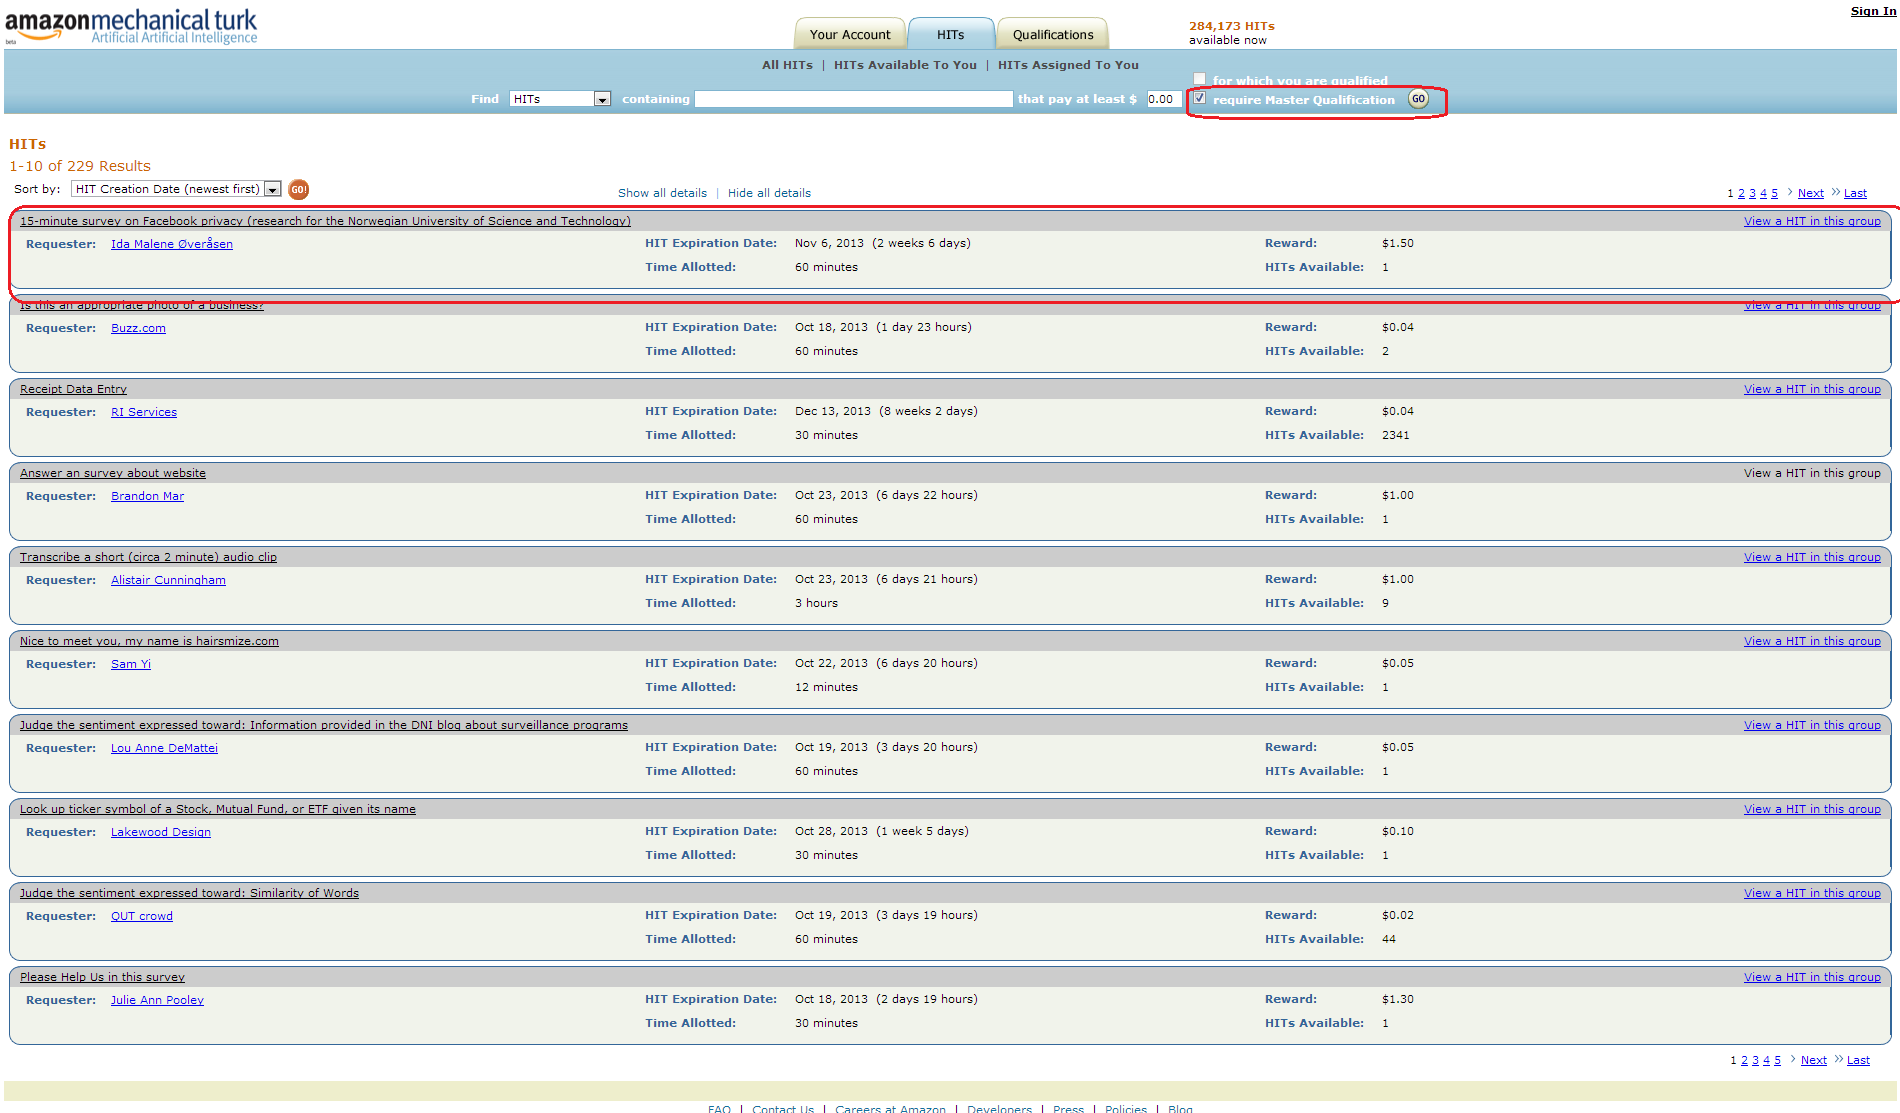
\includegraphics[width=1\textwidth]{hitout.png} }
\caption[Our HIT is published]{\textbf{Our HIT is published.} This figure shows our HIT in the list of all HITs available that requires "Master Workers".} 
\label{fig:hitout}
\end{figure}

We mainly wanted to distribute our survey on AMT, both to try it out as a research tool and because of it's high diversity. But in addition to distributing the survey on AMT, we decided to also share it with our friends on Facebook. We wanted to reach out to a even wider audience, as well as making our Facebook  friends aware of their settings. Most of our Facebook friends mainly consist of fellow students, with a high technical knowledge. We were not depending on Facebook to give us many answers. We were hoping for at least 30 respondents from Facebook, but we got 77 respondents and were amazed of the outcome. We posted it and a few times during the 3 weeks the survey was out, we commented on it so it would appear on top of our friends' News Feeds. Three of our friends even chose to share it on their Facebook. This was probably one of the reasons we got so many answers. We posted it on Facebook a few days later than the HIT was published on AMT.  

\begin{figure}[h!]
\centering
\fbox{
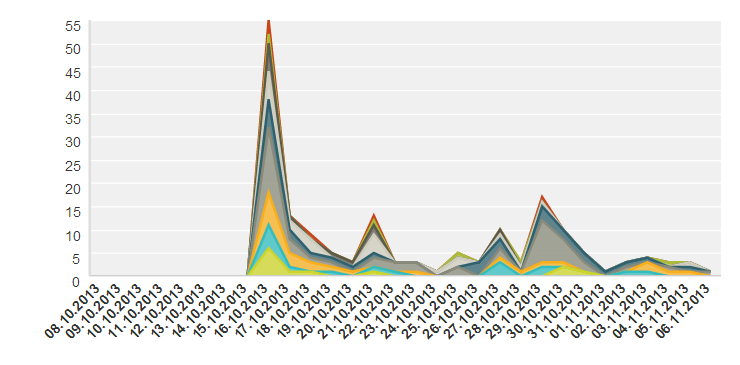
\includegraphics[width=1\textwidth]{answersamt.png} }
\caption[Daily distribution of number of answers from AMT]{\textbf{Daily distribution of number of answers from AMT.}} 
\label{fig:answersamt}
\end{figure}

\begin{figure}[h!]
\centering
\fbox{
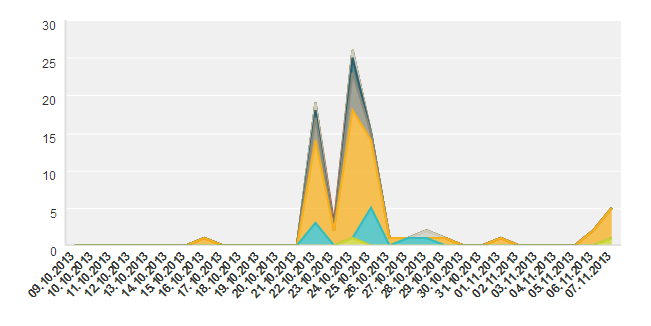
\includegraphics[width=1\textwidth]{answersfacebook.png} }
\caption[Daily distribution of number of answers from Facebook]{\textbf{Daily distribution of number of answers from Facebook.}} 
\label{fig:answersfacebook}
\end{figure}

\fref{fig:answersamt} and \fref{fig:answersfacebook} shows the daily distribution of number of answers, respectively from AMT and Facebook. You can see from \fref{fig:answersamt} that we had the highest peak in responses the day it was published on AMT. The first day we had 55 unique answers, and the second day it dropped to 13 answers. The number of responses varied during the rest of the period, as the figure shows. 

\subsection{Feedback on the Survey}
We got a lot of positive feedback on our survey from Facebook friends. Many have liked it, and many have commented on it. The comments focused mainly on the eye opening aspects of the survey and that it was informative. Some said the survey made them have a clean-up of their settings. Some mentioned that they though they had good control over their settings, but after taking the survey they realized that this was not the case. They became aware of something they did not know. Overall, the feedback was very positive. As mentioned above, 3 of our Facebook friends chose to share the survey further, and this suggests that they were pleased with it and thought it was good and informative. 

Our survey has also been mentioned in forums on for example mturkform.com and mturkgrind.com. Most of the comments regarding our survey on these forums are about the time consumed taking the survey. The comments we got from mturkforum was: \textit{"Time 5 min 35 sec - slow b/c I wanted to learn more about FB privacy..."} and \textit{"Took 8 minutes, light writing but very simple."}
The comments from mturkgrind was: \textit{"About 5 minutes"} and \textit{"Took 8 minutes, very simple and probably could do it in less time. Light writing"}


\section{Survey Results}
%Hvor mange svar vi fikk og sånn
%hvor lenge den lå ute på amt
%Hvordan vi har gått gjennom resultatene, hva vi har fokusert på og hvorfor!

\begin{figure}[h!]
\centering
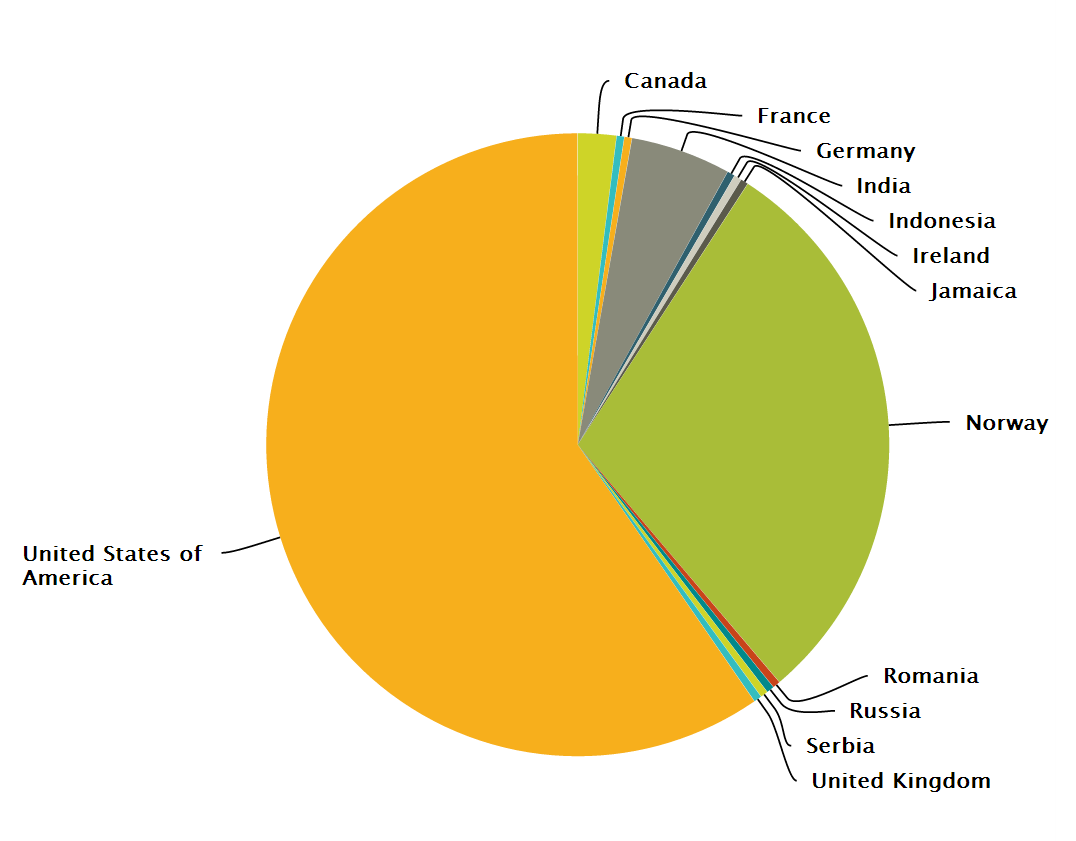
\includegraphics[width=1\textwidth]{land.png}
\caption[Distribution of the participant's country of origin]{\textbf{Distribution of the participant's country of origin.} This graph shows the distribution of the participant's country of origin. Most of the participants are from the United Stated of America and Norway.} 
\label{fig:land}
\end{figure}


\subsection{Demographics}

\begin{figure}[h!]
\centering
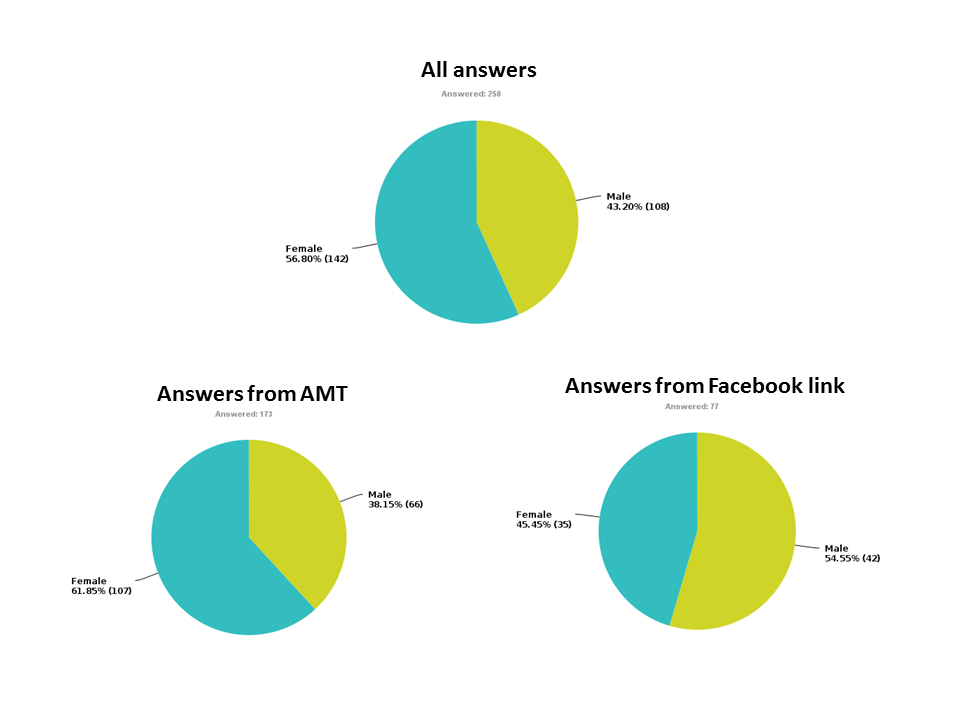
\includegraphics[width=1\textwidth]{gender.png}
\caption[Gender distribution]{\textbf{Gender distribution}. This graph shows the overall gender distribution (on the top), gender distribution from AMT (to the left) and the gender distribution from the Facebook link (to the right).} 
\label{fig:gender}
\end{figure}

As mentioned before, we distributed our survey on two platforms; Amazon Mechanical Turk (AMT) and Facebook. In total we received 250 responses from 13 different countries. As you can see in \fref{fig:land}, the distribution of countries was mainly divided between two, the United States of America and Norway. Other countries were also represented; Canada, France, Germany, India, Indonesia, Ireland, Jamaica, Romania, Russia, Serbia and United Kingdom. 77 of the 250 responses were collected through the Facebook link, and out of these 77 people 96\% (74 people) were from Norway. 173 of the 250 respondents took the survey via Amazon Mechanical Turk, and out of these people 85,5\% (148 people) were from the United Stated of America. 

\paragraph{}
The majority of the total respondents were female. They accounted for 56,80\% of the responses, which is 142 responses. This means that 43,20\% of the total respondents were male, with a 108 responses. We saw a difference in the gender distribution from the Facebook link and from AMT. On AMT 38,15\% were men, and 56,80\% were female. On Facebook 54,55\% were male, and 45,55\% were female. In other word the majority of respondents on AMT were females, in contrary to Facebook, were the majority of respondents were men. The different gender distributions are shown in the \fref{fig:gender}.
 
\paragraph{}
Among the participants, the age ranged betweetn 19 and 76. The average age was 31. The average age of the AMT participants (33 years old) were higher than the average age of the Facebook participants (27 years old). When we looked at the total income of the household per year and employment status, we found a wide range of variety among the participants. We had several participants in each group of income. Although the majority of the participants were employed for wages or students, all of the other employment status' was represented. This was consistent with former studies of AMT users \cite{incentivesAmt}. 


\subsection{Never Checked Facebook Privacy Settings During the Last Year}

\begin{figure}[h!]
\centering
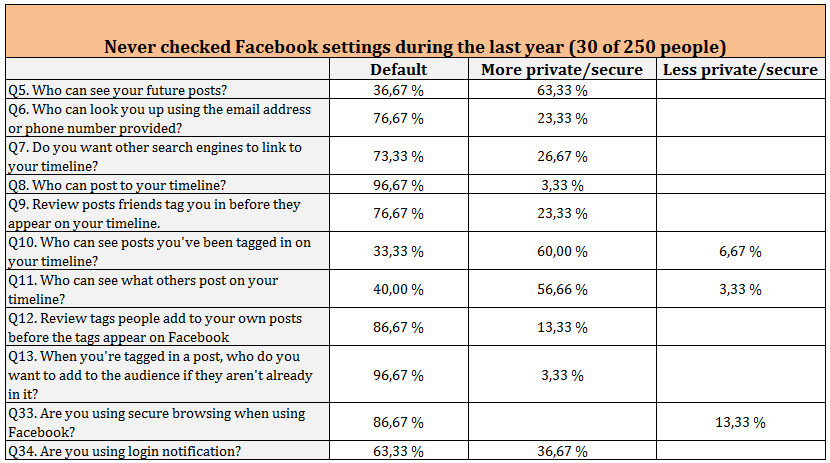
\includegraphics[width=1\textwidth]{nevercheckedtable.png}
\caption[Never checked Facebook privacy settings during the last year]{\textbf{Never checked Facebook privacy settings during the last year.} Forklare hva figuren viser.} 
\label{fig:neverchecked}
\end{figure}

30 of the people who answered our survey stated that they have never checked their privacy settings during the last year. Even though they have not checked their privacy settings during the last year, most of them have done some changes to their settings before the previous year. The reason for this assumption is that their settings differ from the default settings.  
The average number of friends for the people who have never checked Facebook privacy settings during the last year is 162, and their average age is 39. 

In \fref{fig:neverchecked} you can see a percentage distribution over Facebook settings among the people who have never checked their Facebook privacy settings during the last year. We have divided them into tree categories; "Default", "More secure", and "Less secure". You end up under the category "Default" if your setting is similar to the default setting anno 2013. See section \ref{subsec:default2013} for more detailed description of the default settings on Facebook. You end up under the "More secure" category if you have changed the default setting to a more secure setting. The "Less secure" is for those who have made changes to their setting which is less secure than the default setting. 

The majority of these users are active users, since 67\% of them checks their Facebook page at least once a day. 

60\% of the people who had never checked their Facebook privacy settings during the last year \textit{did not} consider changing their privacy settings after reviewing them. 40\% of them wanted to make their privacy settings more private. 

We have a quote from a 67 year old woman that took our survey (with Ph.D and only 5 Facebook friends) that emphasised many user's unawareness when it comes to different Facebook settings: "Now you have scared me. I am alone and afraid".

\subsubsection{App awareness}
73,33\% of these 30 respondents were aware of the fact that all apps on Facebook access their basic information. Less of them were aware that many apps post on your behalf (56,6\%). \fref{fig:appawarenessneverchecked} shows the percentage distribution from four of the app awareness questions. The two on top shows the ones just mentioned respectively. As you can see, the amount who answered "No" increased drastically on the last two questions. The third question asks for the users awareness regarding the fact that some apps access your friends' private information, and the fourth and last regard the fact that some apps have access to relational information (such as private chat messages). 

\begin{figure}[h!]
\centering
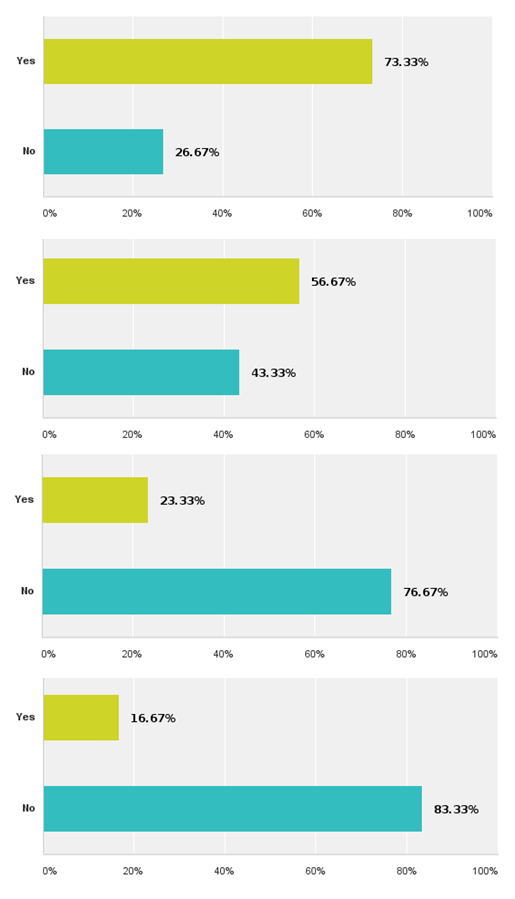
\includegraphics[width=1\textwidth]{q26-29AppAwareness.png}
\caption[The distribution showing app awareness among the 30 respondents that have never checked their Facebook settings during the last year]{\textbf{The distribution showing app awareness among the 30 respondents that have never checked their Facebook settings during the last year.} Showing the distributions of the answers to question 26-29 among those that have never checked their Facebook settings during the last year.} 
\label{fig:appawarenessneverchecked}
\end{figure}


\subsection{Checks Facebook Privacy Settings "Once a month" or "Once a week or more"}

\begin{figure}[h!]
\centering
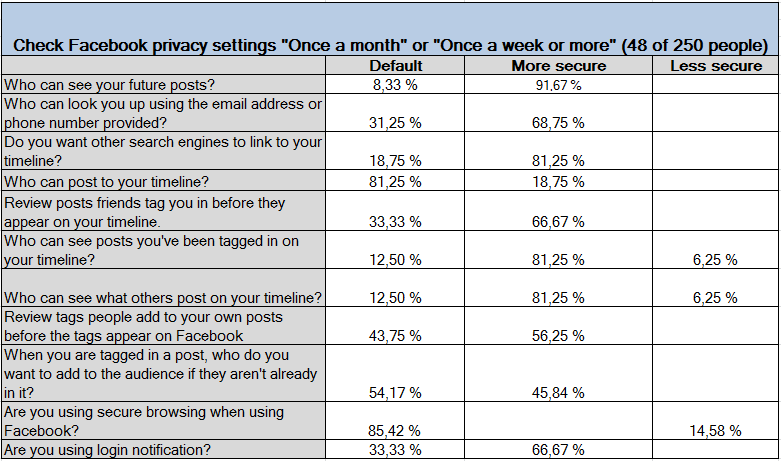
\includegraphics[width=1\textwidth]{checkonceaweekormoretable.png}
\caption[Checks Facebook privacy settings "Once a month" or "Once a week or more"]{\textbf{Checks Facebook privacy settings "Once a month" or "Once a week or more".} Forklare figuren mer nøye her} 
\label{fig:onceaweekormore}
\end{figure}

48 of the people who answered our survey stated that they check their privacy settings "Once a month" or "Once a week or more". The average number of friends for these people is 416, and their average age is 28,5. 

In \fref{fig:onceaweekormore} you can see a percentage distribution of what kind of settings the people who check their privacy settings "Once a month" or "Once a week or more" have. We have divided them into the same categories as above; "Default", "More secure", and "Less secure".  

85\% of the people who checked their Facebook privacy settings "Once a month" or "Once a week or more" during the last year, has checked their Facebook page at least once a day during the last month. This indicates that the majority of those who check their settings frequently are also very active Facebook users. 

70,83\% of these people did not consider changing privacy settings after reviewing them. 27,08 \% wanted to make their privacy settings more private, and 2,08\% considered changing them to more public. 


%12 of the 48 people in this category answered yes on the question whether or not facebook had affected their personal life negativally. Half of these had situations with friends posting unwanted pictures (av forskjellige grunner) of them.

%One guy: Two accounts; one under a pseudonym for friends only and on with strict settings for the rest of the world. "Privacy is important to me. It is meaningless not to give others the same courtesy" - Random guy with 420 friends that are 43 years old. 
\subsubsection{App awareness}
72,92\% of these 48 respondents were aware of the fact that all apps on Facebook access their basic information. A larger number of these respondents were aware that many apps post on your behalf (81,25\%). \fref{fig:appawarenessonceaweek} shows the percentage distribution from four of the app awareness questions. The two on top shows the ones just mentioned respectively. As you can see, the share who answered "No" increased on the last two questions. The third question asks for the users awareness regarding the fact that some apps access your friends' private information, and the fourth and last regard the fact that some apps have access to relational information (such as private chat messages).  

\begin{figure}[h!]
\centering
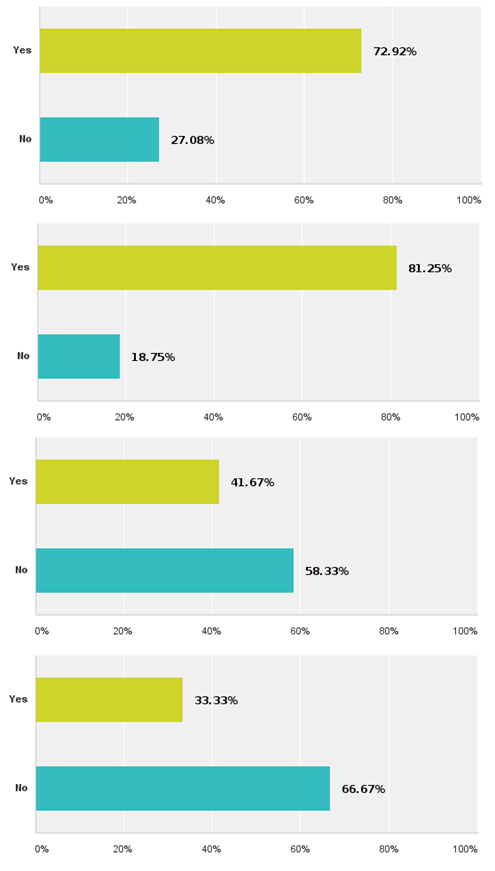
\includegraphics[width=1\textwidth]{q26-29OnceAWeek.png}
\caption[The distribution showing app awareness among the 48 respondents that checks their Facebook settings "Once a month" or "Once a week or more"]{\textbf{The distribution showing app awareness among the 48 respondents that checks their Facebook settings "Once a month" or "Once a week or more".} Showing the distributions of the answers to question 26-29 among those that check their Facebook settings "Once a month" or "Once a week or more".} 
\label{fig:appawarenessonceaweek}
\end{figure}


\subsection{Comparing the ones who have "Never checked their Facebook privacy settings during the last year" and the ones who checks "Once a month" or "Once a week or more"} 

\subsubsection{Activity level.}
The majority of both groups checks their Facebook page at least once a day. The percentage is a little bit higher for the people who have checked their privacy settings "Once a month" or "Once a week or more" during the last year. 85\% of them checks their Faceook page at least once a day, in contrast to the other group (who have never checked their settings during the last year) with 67\% checking their Facebook page at least once a day. This indicates that the ones who have never checked their settings during the last year does not refrain from doing this because they are inactive users. One assumption for this may be that the users are unaware of the settings. 40\% of them stated that they wanted to make their settings more private after taking the survey. This backs up the assumption about unawareness.  



\subsubsection{More secure settings for those who check their settings more often?}
If we compare \fref{fig:neverchecked} and \fref{fig:onceaweekormore}, we see a clear difference in percentage that have changed from default to a more secure option. The percentage is much higher for all settings listed for those who checks frequently. Some of the settings shows a remarkable difference between the groups. We want to accentuate the settings that concern interdependent privacy. When we look at the setting "Review posts friends tag you in before they appear on your timeline" for the ones that never checked during the last year, only 23,33\% have changed to a more secure option. For the ones that check frequently, 66,67\% have changed to a more secure option. Another example is the setting "Review tags people add to you own posts before the tags appear on Facebook" where 13,33\% of the ones who never have checked their settings during the last year changed to a more secure option. On the contrary, as many as 56,25\% of the frequent settings-checkers have changed to a more secure option.

\subsubsection{Considered changing settings.}
The percentage of those wanting to make their settings more private is higher for those who have never checked settings during the last year with 40\% of the group. Only 27\% of the frequent setting-checkers wanted to make their settings more private. 
None of the people who have never checked their settings during the last year wanted to make their settings more public, unlike the other group (those who check "Once a month" or "Once a week or more") where 2\% actually considered changing them to more public. Overall the frequent settings-checkers were more pleased with their settings than the once who had never checked them during the last year. 70\% of the frequent settings-checkers did not consider changing their settings after reviewing them. Although the ones who have never checked their settings during the last year have far less secure settings than the other group, 60\% of them did not consider changing their settings either. 

\subsection{Comparisons with Previous Surveys} 
In the article "Analyzing Facebook Privacy Settings: User Expectations vs. Reality" mentioned in section \ref{sec:relatedwork_facebookprivacy}, they found that modified privacy settings match the users expectations only 39\% of the time. In our case this number is much higher, 65,6\% stated what they did not consider changing their privacy settings after reviewing them. This is an interesting observation. The previous research was done in 2011, and a lot has changed since then with regard to privacy settings. One assumption is the ongoing attention towards online security. With the media trying to make people aware of how easy it is to access ones information on the web. 

In the other article mentioned in \ref{sec:relatedwork_facebookprivacy}, "Facebook privacy settings; Who cares?" they found that among the majority both genders were equally confident in changing their Facebook privacy settings. Our survey backs up this finding to some extent. The majority of both females and males have changed their settings to a more private option, but our research shows that females focus more on who can see their posts and posts they have been tagged in and who can look them up. 81\% of the females have changed the settings "Who can see posts you've been tagged in on your timeline?" and "Who can see what other's post on your timeline?" to a more private option. In both of these settings, this is almost 10\% more than for males. In contrary, males have a larger focus on security, with more secure options on settings like "Login notification" and "Secure browsing". 

\subsection{Users' personal experience}
Out of the 250 respondents 11 answered yes on the question "Have you ever experienced that your use of Facebook has affected your professional life?". 3 of these 11 have had their professional life affected in a negative way, and 8 was affected in a positive way. 
50 of the 250 respondents stated that their use of Facebook had lead to uncomfortable situations, for example concerning unpleasant messages and/or inappropriate comments or pictures. The majority of the situations concerns unwanted pictures (where they do not look good) shared beyond their preferred audience and inappropriate comments on pictures of them. Some also mention cases of stalking. Some of the comments are shown below:

\begin{itemize} 
\item "\textit{I had a friend I parted ways with harass me on Facebook by threatening messages, posts to photos about me, etc. I also had sexual harassment over Facebook message by an ex boyfriend, inappropriate comments and propositions I was not interested in.}"
\item "\textit{Before I changed my settings, someone posted a picture of me that I did not want to share with everyone else.}"
\item "\textit{An ex girlfriend was using Facebook to get information about me and my friends.}"
\item "\textit{I shared (public) a photo from a friends timeline which he had posted to a limited set of friends, he got mad.}"
\item "\textit{I have many younger friends on Facebook (underage), and I would like to be a good role model. So sometimes there have been pictures of me consuming alcohol, and I don´t want my younger friends to see that. I now have customized my settings, so they only see my personal posts which dosen´t include alcohol/smoking etc.}"
\item "\textit{Someone commented something on a photo I was tagged in that I don't want everyone to know about me}"
\item "\textit{I girl posted a naked photo of me.}"
\item "\textit{Just pictures of me not looking my best being posted by friends who then tag me and suddenly everyone - friends of friends, etc. can see the pics. It wasn't disasterous or inappropriate, but those weren't pictures I wanted old classmates from high school to look at (unless we are friended on FB)}"
\end{itemize}

39,6\% of the total respondents have blocked one or more person due to uncomfortable situations or harassment. 

To see how much a person values their privacy, we asked them to state on a scale from 1 to 5 to what degree they care about what is published about themselves. 1 is "I don't care at all. Everything can be public" and 5 is "I untag and hide everything that is published of me". The majority (35,6\%) answered 3 on the scale.  When people were asked to elaborate on this topic, the comments ranged from "I don't trust the Internet" to "I don't untag everything, because the point of the site is to be social". Many says that they frequently untag photos they do not want others to see. One of the respondents said "It's a tricky dilemma, because when you untag you also loose control over what happens with the picture/post."

From our results, it seem like people care more about what they post of others, than what is posted about themselves. When we asked them to what degree they are selective about what they post about others on a scale from 1 to 5, where 1 is "I am not selective at all, I post everything" and 5 is "I never post anything about anyone", the majority answered 4. This shows that people are very selective when it comes to posting things about others.

\subsection{Interdependent Privacy}

A big part of our survey focus on apps and the issues related to apps which concerns interdependent privacy. When installing an app on Facebook, most apps ask for permission to access additional information in addition to your basic information (name, profile picture, cover photo, gender, networks, username, user ID, your list of friends, and any information you choose to make public). We wanted to map the awareness of the respondents when it came to apps, and to what degree they knew about the information apps access. We also wanted to find out whether or not the respondents had knowledge about the term interdependent privacy. We asked the question "Do you have any idea about what interdependent privacy can mean in regard to Facebook?" both before and after the app-related questions. We specified in the question that they were not allowed to use Google or any other search engine to find the answer, and if they did not know the answer it would be preferable for us if they skipped the question. It would not be of any value for us, if they searched for the "definition". We wanted to see if people could come up with their own idea of the term. It was 136 people that skipped or answered that they did not know what it was, both before and after the app-related questions. 69 of the respondents skipped the first question, but answered the second one. Even though everything was not entirely correct, a lot of people seemed to have gotten some idea of what the term evolves around after answering the question about apps. \tref{tab:thoughtonintpriv} shows some of the answers, both before and after the app-related questions.   

%høy security/privacy = høy int. priv?

\begin{center}
\begin{longtable}{ | p{6cm} | p{6cm} |}
    \caption{\label{tab:thoughtonintpriv}Peoples thoughts of what is meant by interdependent privacy before and after answering questions about privacy issues regarding the use of Facebook apps.} \\
    \hline
\textbf{Q24. Do you have any idea about what interdependent privacy means?} & \textbf{Q31. Do you have any idea about what interdependet privacy means after answering questions regarding privacy issues using Facebook apps?} \\ 
\hline
I have no idea what interdependent privacy means. It almost does not make sense to put those two words together. If you have privacy, it should not depend on another party to make it private. That defetes the whole purpose of "private". &  Hmn. I guess it makes sense now, seeing that apps can do that to people who are friends.\\ 
    \hline
I would image it relates to one person's privacy being compromised or supported by another user's privacy settings. & Yes, I understand what it means now. If a friend of mine permits an app to access their info then they have a certain amount of access to my info.\\ 
    \hline
I think it's when my picture is visible to only friends but then a friend of mine reshares it, so I have to rely on that friend to keep my stuff private too. &  I think I was close to right. Relying on others' settings to keep my privacy.\\ 
    \hline
I think it means that people you allow to see things can also allow others to see it if they chose to, with or without your permission but I am not sure about this. & I think that it means if you give an app permission to use your information, the app can then use the information in any way it wants to. This is why I do not use any apps because I do not trust them period.\\
    \hline
I think it has to do with other sites and apps allowing you to sign into or register for accounts using your facebook account.  You would now have another set of privacy policies to review and how the two sites work together & Apps you use can disregard your privacy settings with facebook and play by tehir own rules - so I have to be much more diligent.\\
	\hline
I think it means that people you allow to see things can also allow others to see it if they chose to, with or without your permission but I am not sure about this. & I think that it means if you give an app permission to use your information, the app can then use the information in any way it wants to. This is why I do not use any apps because I do not trust them period.\\
    \hline
It's something about where someone else saying something (like Bob saying "Bob is at the restaurant with Mike") can reveal information about another person (in this case, that Mike is at the restaurant). & Maybe it's: Facebook taking other people's info based on something I do. \\
    \hline
    My privacy can be affected by those I share with. Just because I make something private does not mean that my friends won't pass it along, making it no longer private. & You are not the only person in control of your privacy. If you don't use the right settings, other people can share information you think is private.\\ 
    \hline  
I have no control over what info my friends share about me & (Skipped) \\
    \hline
Nope. I will for sure google it now. & That it´s obv. not only facebook who can access my privacy settings, that this so called privacy is interdependet and I am in charge of setting those settings myself if I don´t want it to be that interdependent. \\
    \hline
What others can do to your privacy if you "let them"? & Yes. what concerns your privacy that you dont know of, that your friends do to your privacy ish.\\ 
    \hline  
My privacy depends on others & The apps are allowing people to see things that are private. It's interdependent on FB.\\ 
    \hline
I would say it means it depends on what others would post or say about you, or give out your private things. & You can control what you share, but not what others do or say that may infringe on your privacy.\\ 
    \hline 
No & Getting access through games and friends. \\ 
    \hline
(Skipped) & My privacy setting depends also on other users, with the help of apps. I think this is what interdependent privacy means.\\ 
    \hline
(Skipped) & Maybe other apps can take information from your friends without their knowing.\\ 
    \hline    
(Skipped) & It seems to be privacy independent from privacy settings. It appears apps can override general privacy settings.\\ 
     \hline
(Skipped) & That apps I put on my FB page can access my friend's accounts, information and activities. I am always very careful to select "ONLY ME" when they ask whose wall they can post to - but I wasn't aware that apps were independently able to access the information of my friends without my consent.\\ 
     \hline 
(Skipped) & I think that it means that the apps that I use can have an effect on my friends privacy.\\ 
     \hline     
    \end{longtable}
\end{center}

An issue discussed in the paper "Third-Party Apps on Facebook: Privacy and the Illusion of Control" \cite{thirdPartyApps} is the importance of user control of apps' data access, and that it should be made clear to the user what information they give the apps permission to access. In this paper, they conclude that it is often unclear for the users what information they agree to share, and that apps often ask for permissions that are in conflict with their privacy settings. We wanted to see if the users were aware of what information apps may ask for, and how much information they may agree on sharing (not just about themselves). 

In the apps settings, one can see a list of all the apps the user have connected to Facebook. \fref{fig:appsyouuse} show the amount of apps the respondents have. The distribution is close to even for all the alternatives. 86,8\% of the total respondents have at least one app connected to their Facebook. We can see that a higher percentage of the respondents have more than 30 apps in comparison to none. 

\begin{figure}[h!]
\centering
\fbox{
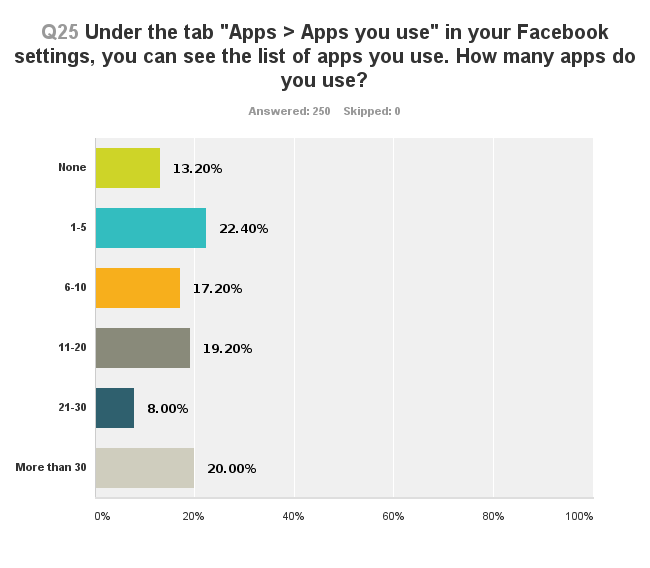
\includegraphics[width=0.8\textwidth]{appsyouuse.png}}
\caption[Question 25 - Displaying number of apps you use]{\textbf{Question 25 - Displaying number of apps you use.} After receiving 250 answers, this is the summary of the answers to question 25 asking for the number of apps the user use.} 
\label{fig:appsyouuse}
\end{figure}

\fref{fig:appsaccessbasicinfo}, \fref{fig:appspostonyourbehalf}, \fref{fig:appsaccesstofriendsinfo} and \fref{fig:appsaccessrelationalinfo} shows the results from question 26, 27, 28 and 29, where we ask the respondents about their awareness regarding the information apps requests. The two first figures shows that the majority of the respondents were aware of the facts presented. The two last figures, on the other hand, shows that the majority were unaware of the permission requests. The two first questions are more visible for the users, it is stated many times that all apps access your basic and public information, and the users experience apps posting both on their behalf and on friends' behalf (for example Spotify posting playlists or songs you have listened to). The two last questions is more hidden from the users, because nothing is posted or viewable etc. The users is not notified when the apps access this information, and therefore have no specific idea what is retrieved, when it is used, and for what purpose. We therefore think it is less knowledge about these permission requests. 

\begin{figure}[h!]
\centering
\fbox{
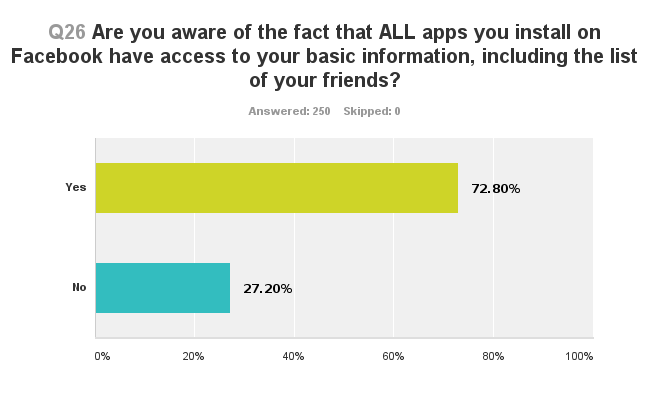
\includegraphics[width=0.8\textwidth]{appsaccessbasicinfo.png}}
\caption[Question 26 - Displaying the awareness of the fact that all apps access your basic information]{\textbf{Question 26 - Displaying the awareness of the fact that all apps access your basic information.} All apps you install on Facebook have access to your basic information, including the list of your friends. 72,80\% of the respondents were aware of this.} 
\label{fig:appsaccessbasicinfo}
\end{figure}

\begin{figure}[h!]
\centering
\fbox{
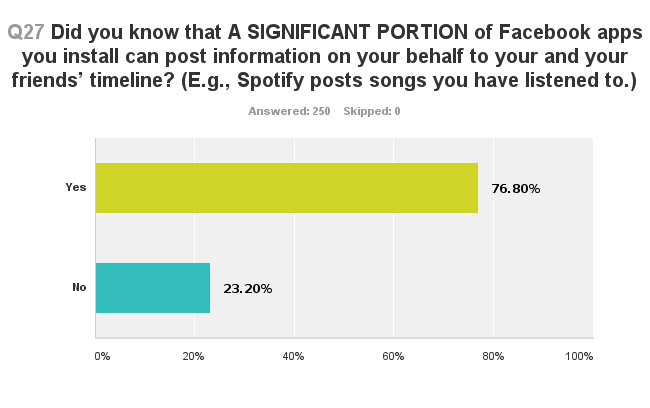
\includegraphics[width=0.8\textwidth]{appspostonyourbehalf.png}}
\caption[Question 27 - Displaying the awareness of the fact that a significant portion of apps post on your behalf]{\textbf{Question 27 - Displaying the awareness of the fact that a significant portion of apps post on your behalf.} A significant portion of apps you use on Facebook post to your timeline and your friends' timeline on your behalf, for example Spotify posting songs you have listened to. 76,8\% of the respondents were aware of this.} 
\label{fig:appspostonyourbehalf}
\end{figure}

\begin{figure}[h!]
\centering
\fbox{
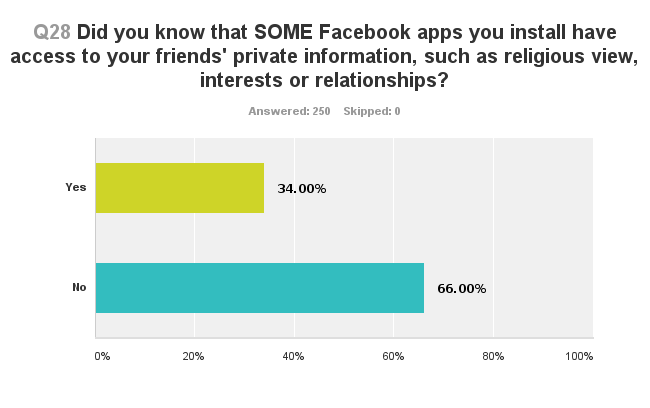
\includegraphics[width=0.8\textwidth]{appsaccesstofriendsinfo.png}}
\caption[Question 28 - Displaying the awareness of the fact that some apps access your friends' private information]{\textbf{Question 28 - Displaying the awareness of the fact that some apps access your friends' private information.} Some apps you use on Facebook access your friends' private information, such as religious view, interests and relationships. 34\% of the respondents were aware of this.} 
\label{fig:appsaccesstofriendsinfo}
\end{figure}

\begin{figure}[h!]
\centering
\fbox{
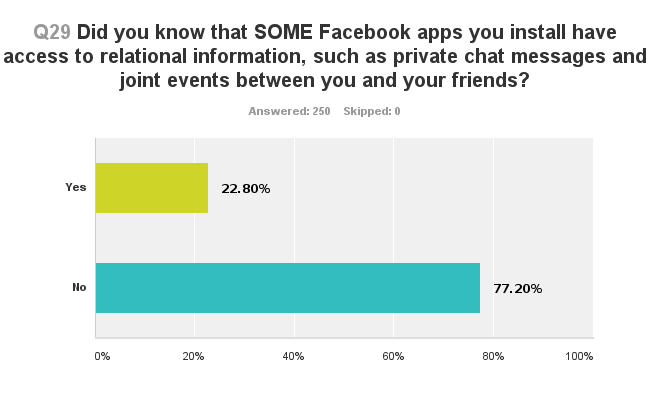
\includegraphics[width=0.8\textwidth]{appsaccessrelationalinfo.png}}
\caption[Question 29 - Displaying the awareness of the fact that some apps access relational information]{\textbf{Question 29 - Displaying the awareness of the fact that some apps access relational information.} Some apps you use on Facebook access relational information, such as private chat messages and joint events between you and your friends. 22,8\% of the respondents were aware of this.} 
\label{fig:appsaccessrelationalinfo}
\end{figure}

\begin{figure}[h!]
\centering
\fbox{
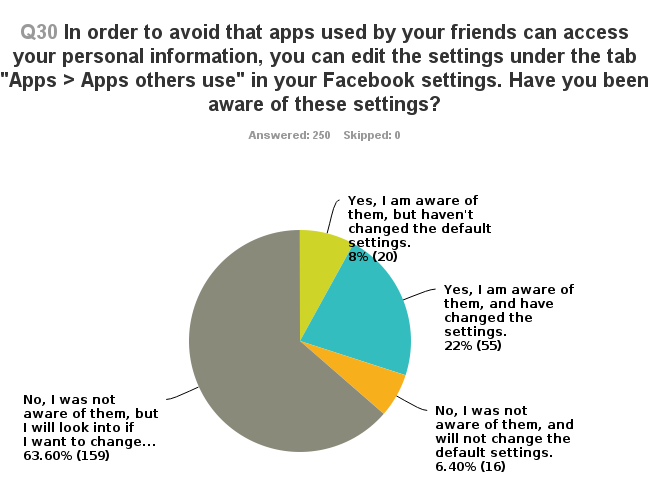
\includegraphics[width=0.8\textwidth]{appsothersuse.png}}
\caption[Question 30 - Displaying the awareness of the setting "Apps others use"]{\textbf{Question 30 - Displaying the awareness of the setting "Apps others use".} Under the setting "Apps others use" the user can edit what information about you apps used by your friends can access. 70\% of the respondents were NOT aware of this setting.} 
\label{fig:appsothersuse}
\end{figure}

We wanted to find out whether or not people using many apps had more or less knowledge when it came to the app-related questions, than people using few apps. \textit{Our hypothesis were that the ones with many apps have less knowledge about the privacy issues related to apps}. The reason for this assumption is that we thought if these people were aware of all the permissions they agree/agreed on, they would not have had that many apps to begin with (because of the privacy breach apps cause). On the other hand, we thought that those with few apps had more knowledge about the privacy issues related to apps, and therefore chose to refrain for installing apps and/or are frequently deleting the apps not in use.
\fref{fig:manyappsandfewapps} shows the results of this comparison. On question 26 the distribution is close to equal for those with many apps (21 apps or more) and those with few (5 apps or less). This is a relatively common known fact, because information about this is stated on the top of the app settings, as well as always on top of the list when installing an app. Question 27 shows that the people with many apps were more aware of the fact that a significant portion of apps post on your behalf. We think the reason for this is that the people who frequently use apps have more experience when it comes to apps posting on their behalf, and this makes them more aware of this fact. When apps post on behalf of a user, it is shown on your timeline. This is something the user experiences hands on. In addition to this, people who use many apps sees the permission requests from Facebook more frequently. Question 28 and question 29 on the other hand, are not visible for the naked eye. Although, this is stated in the permission request, it is never visible for the user what information is accessed and retrieved by the apps. The percentage of people aware of the facts presented in question 28 and question 29 is higher for those with few apps than for those with many apps. This backs up our hypothesis. The last question (30) concerns the setting "Apps others use" found under the App tab in your Facebook settings. Here you can choose which information your friends' apps can access. From our results you see that 37,08\% of those with few apps were aware of the existence of this setting. Almost 10\% less of the ones with many apps were aware of it. This also backs up our hypothesis that the ones with few apps are to a larger extent aware of the privacy issues related to apps and the settings that exist. 

\paragraph{}
Question 30 asks not only for a simple "Yes" or "No" answer to whether or not they are aware of the setting "Apps others use". The possible answers for the question is "Yes, I am aware of them, but I haven't changed the default settings", "Yes, I am aware of them, and have changed the settings", "No, I was not aware of them, and will not change the default settings" and "No, I was not aware of them, but will look into if I want to change my settings now". The latter option was significantly higher for those with many apps, which means a higher portion of those with many apps were unaware of this setting and dissatisfied with the configuration of this setting, compared to the ones with few apps. Another observation is that the alternative "Yes, I was aware of them, and have changed the settings" is higher for those with few apps. These results are shown in \fref{fig:appsothersusemanyfew}. These results also back up our hypothesis. 

\begin{figure}[h!]
\centering
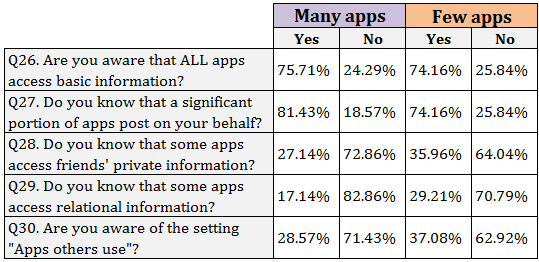
\includegraphics[width=0.8\textwidth]{awareness(manyappsandfewapps).png}
\caption[App awareness - Comparing those with many app and those with few apps]{\textbf{App awareness - Comparing those with many app and those with few apps.} Percentage distribution of the answers to all of the app questions differentiating the 70 people with many apps (21 apps or more) and the 89 people with few apps (5 or less).} 
\label{fig:manyappsandfewapps}
\end{figure}

\begin{figure}[h!]
\centering
\fbox{
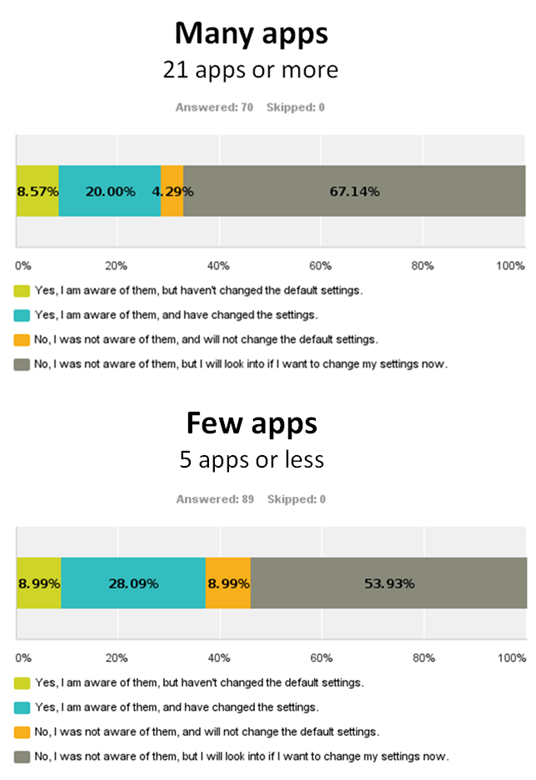
\includegraphics[width=0.6\textwidth]{appsothersusemanyfew2.png}}
\caption[Awareness of the setting "Apps others use" - Comparing those with many app and those with few apps]{\textbf{Awareness of the setting "Apps others use" - Comparing those with many app and those with few apps.}} 
\label{fig:appsothersusemanyfew}
\end{figure}



